\begin{figure*}[t]
  \centering
  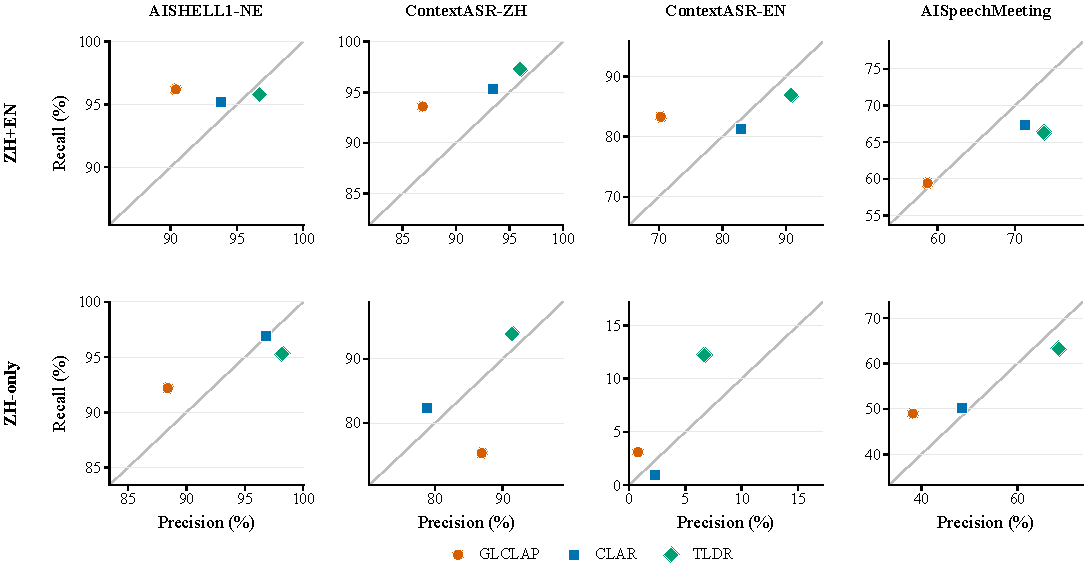
\includegraphics[width=0.98\textwidth]{figure/fig_retrieval_precision_recall.pdf}
  \caption{Precision-recall behavior of hotword retrieval systems. Each panel compares GLCLAP, CLAR, and TLDR on one benchmark under one training regime. TLDR generally shifts the operating point toward higher precision and recall, while CLAR remains competitive on the clean AISHELL1-NE setting. Axes are locally scaled for readability.}
  \label{fig:retrieval_pr}
\end{figure*}

\begin{figure*}[t]
  \centering
  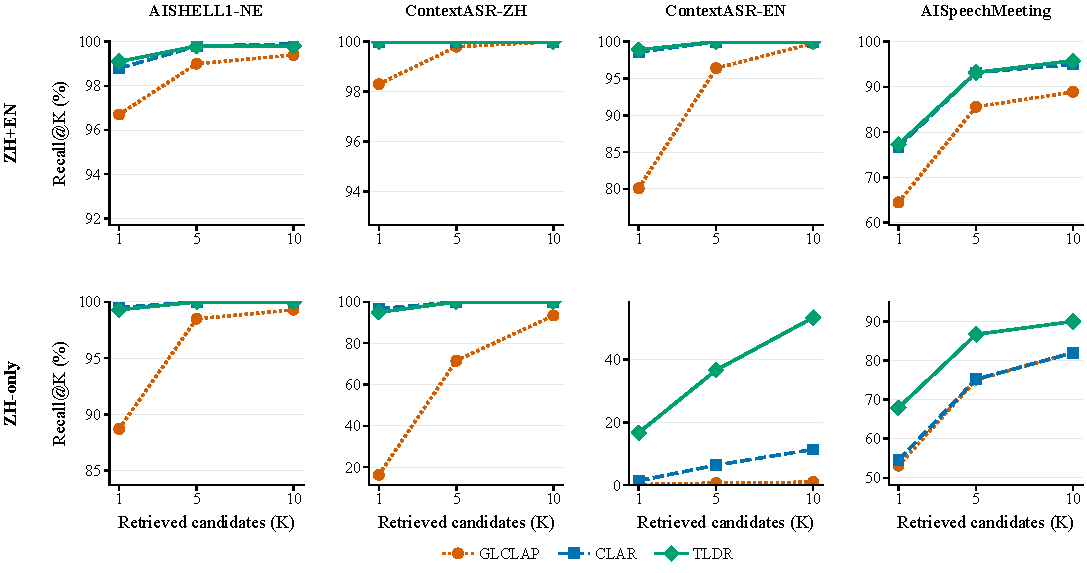
\includegraphics[width=0.98\textwidth]{figure/fig_retrieval_recall_at_k.pdf}
  \caption{Candidate ranking quality measured by Recall@K. While several ZH+EN results saturate at larger K, the ZH-only setting exposes larger differences: TLDR retains substantially higher ranked recall on ContextASR-EN and AISpeechMeeting. Axes are locally scaled for readability.}
  \label{fig:retrieval_ratk}
\end{figure*}

\begin{figure*}[t]
  \centering
  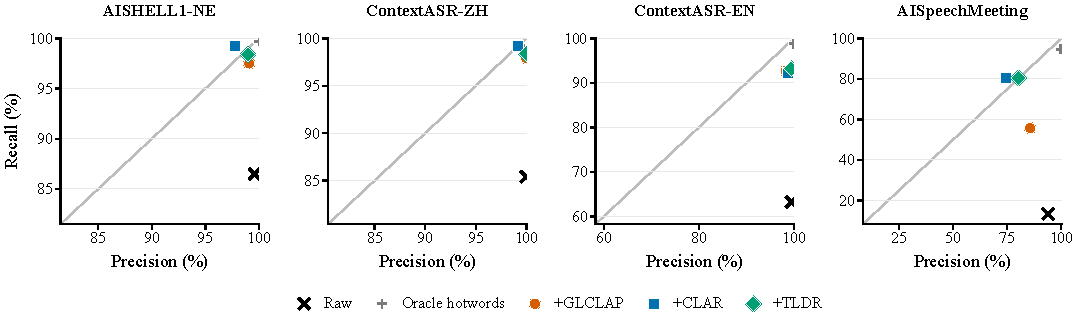
\includegraphics[width=0.98\textwidth]{figure/fig_decoding_precision_recall.pdf}
  \caption{Hotword precision-recall behavior after downstream decoding. Compared with retrieval baselines, TLDR produces a more balanced decoding operating point on the difficult English and meeting benchmarks, which is consistent with the WER reductions in Table~\ref{tab:decoding_main}. Axes are locally scaled for readability.}
  \label{fig:decoding_pr}
\end{figure*}
